Fracture at the atomic scale is a complex process controlled by the local structure of atoms, applied stress, forces between atoms and the strength of atomic bonds.  In order to predict the dynamics of the fracturing process, we are developing graph-based ML algorithms that learn from molecular dynamics simulation data.


\section{Data}
Sandia National Laboratories is providing the MD simulation results that we use as training data for our ML models, as well as a set of Python scripts to facilitate data processing and loading the data into appropriate data structures. Simulations are generated using the LAMMPS code (Large-scale Atomic/Molecular Massively Parallel Simulator)~\cite{PAMD}.  Each LAMMPS run simulates a sample of SiO$_2$ containing approximately 70,000 atoms. The simulations use the reactive force-field potential ReaxFF~\cite{pitman2012dynamics}.

Starting from a crystalline state of stoichiometric quartz, MD initially simulates melting the system for 200~ps, then quenching for 1~ns. The melt-quench procedure is performed using an \emph{NVT ensemble}, meaning that the number of atoms, volume, and temperature are controlled: the density is held constant at 2.2~g/cm$^3$, and the temperature is held constant at 4000~K during the melting phase and then linearly decreased to 300~K (through a velocity scaling procedure) at a constant rate of 3.7~K/ps during the cooling phase.  The system is subsequently equilibrated at 300~K for 200~ps under an \emph{NPT ensemble}, meaning that the number of atoms, pressure, and temperature are controlled. The entire process~\cite{markpres} is illustrated in Figure~\ref{fig:melt_quench}.

\begin{figure}[t]
    \centering
    \noindent
    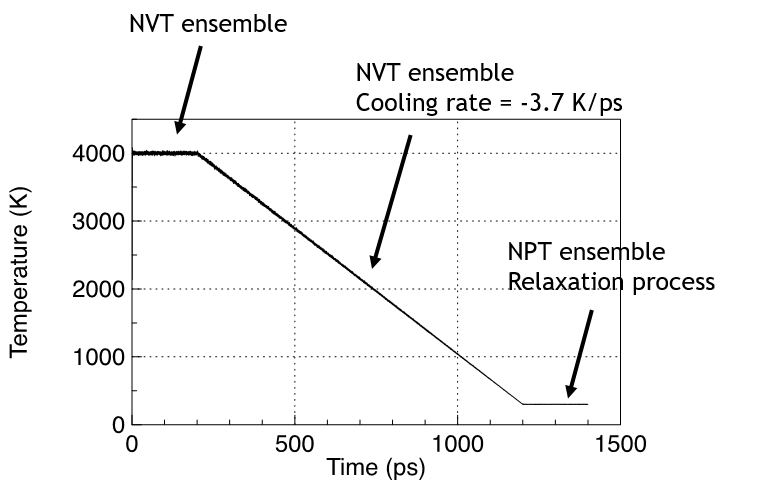
\includegraphics{images/meltquench}
    \caption{Plot reproduced from~\cite{markpres}, showing the temperature schedule used in LAMMPS runs for melting, quenching, and equilibrating the SiO$_2$ sample.}
    \label{fig:melt_quench}
\end{figure}

This procedure generates an amorphous silicate glass of size approximately 15 $\times$ 15 $\times$ 4~nm$^3$, with some variability due to cell relaxation during NPT equilibration dynamics.  The system is loaded in uniaxial tension along the $x$-axis (horizontal), at a constant strain rate of $5\times 10^8$~sec$^{-1}$, for a period of 1~ns.  The resulting strain of 0.5 is sufficient to induce fracture in all simulations. %, and to induce failure as well in some simulations, in which case the run is stopped at that point.

Simulation steps are spaced 0.5~femtoseconds ($0.5 \times 10^{-15}$~s) apart, with snapshots recorded every 2000 steps under loading, representing a spacing of $\Delta t = 1$~ps between snapshots.  The full 1~ns of mechanical loading therefore involves $2 \times 10^6$ simulation steps, or 1000 snapshots. At each snapshot, information recorded for each atom includes $x,y,z$ coordinates, charge, and stress tensor components, and bond connectivity~\cite{markpres}.  This information is supplied in raw form, and is also postprocessed to identify structural properties of the system such as newly formed/broken bonds, SiO$_n$ distribution, and Q$_n$ distribution.

%The silicate is exposed to these conditions following uniform quenching process done at 3.7K/picoseconds. The quenching process is controlled in order to limit the variance in the arrangement of the tetrahedra structure \cite{ebrahem2018influence}. We have four different environmental conditions but all procedures start at equilibrium.

Simulations are run under the following four sets of environmental conditions:

\begin{enumerate}
    \item Dry (vacuum), with periodic boundary conditions in the $x$ direction and free surfaces in the $y$ and $z$ directions. See Figure~\ref{fig:crack_prop}, where the $x$ direction is shown on the horizontal axis.
    \item Dry (vacuum), with fully periodic boundary conditions ($x$, $y$ and $z$ directions).
    \item Wet (H$_2$O in interstices), with periodic boundary conditions in the $x$ direction and free surfaces in the $y$ and $z$ directions.
    \item Wet (H$_2$O in interstices), with fully periodic boundary conditions ($x$, $y$ and $z$ directions).
\end{enumerate}

\noindent
Note that in the example of Figure~\ref{fig:crack_prop}, where there are free surfaces in the $y$ and $z$ directions, fractures typically originate at a surface.  Under fully periodic boundary conditions, where there are no surfaces, fractures must necessarily nucleate within the bulk. For this reason, fully periodic boundary conditions model samples that are far from a surface, where the entire sample can be considered as a bulk material.

For each of the four environmental conditions above, 100 simulations are supplied as training data for our ML algorithms.  Each simulation corresponds to a different configuration, where the distribution of initial velocities is generated using a different random seed.  Running a single one of these simulations requires a total of approximately 10,000 processor hours at Sandia. Without the massively parallel capabilities of LAMMPS, each of these could take over a year to run.  Even with the parallel use of thousands of processors, generating one set of 100 simulations can involve weeks of clock time, motivating the need for rapid surrogate modeling alternatives such as ML.

\section{Graph Representation}
SiO$_2$ may be represented as a network of silicon and oxygen atoms, connected with chemical bonds.  Predicting atomic scale fracture dynamics can therefore be understood as predicting the evolution of the graph that describes this network.

\subsection{Basic Graph Representation}

One straightforward graph representation of the atomic system is as follows.  Consider a graph $G =(V,E)$.  Let each element of the node or vertex set $V$ represent an atom, whether silicon or oxygen.  Let each element of the edge set $E$ represent a chemical bond between two atoms.  The resulting structure is illustrated in Fig.~\ref{fig:basic_graph}.  Note that in this representation, there is additional label information attached to each node, consisting of the atom type: Si or O.

\begin{figure}
\centering
\noindent
    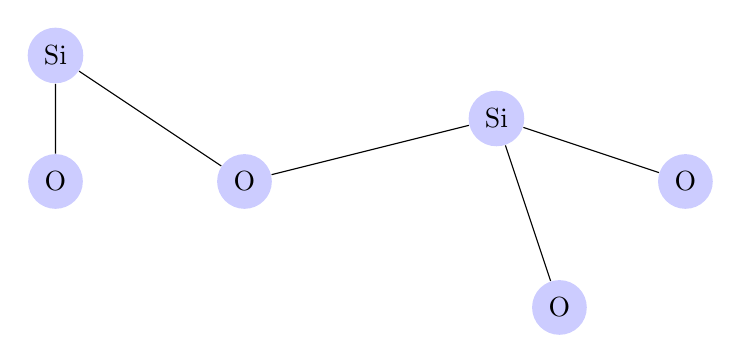
\begin{tikzpicture}
      [scale=.8,auto=left,every node/.style={circle,fill=blue!20}]
      \node (n6) at (1,10) {Si};
      \node (n4) at (4,8)  {O};
      \node (n5) at (8,9)  {Si};
      \node (n1) at (11,8) {O};
      \node (n2) at (9,6)  {O};
      \node (n7) at (1,8)  {O};
    
      \foreach \from/\to in {n6/n4,n4/n5,n5/n1,n2/n5,n6/n7}
        \draw (\from) -- (\to);
    
    \end{tikzpicture}
\caption{Basic graph representation, where nodes denote either silicon or oxygen atoms and edges denote bonds between atoms.}
\label{fig:basic_graph}
\end{figure}

As uniaxial stress is applied to the material, bonds can break and form, whereas atoms are conserved.  Thus, the vertex set remains constant, with size $|V|=n$ given by the total number of atoms in the system, whereas the edge set evolves in time.  We then define $E(t)$ to be the edge set at time step (snapshot) $t$, and $G(t) = (V,E(t))$ to be the graph at time step $t$.

There are significant benefits to having vertices whose identities do not change over the course of the simulation.  When predicting whether or not an atom ends up on the surface of a crack face, it is convenient to able to describe that atom by the same graph element at $t=0$ as at the time of prediction.  A drawback of this representation, however, is the resulting graph size for the samples that we study.  Training an ML algorithm on graph inputs with 70,000 vertices may place excessive demands on computational resources.
    
\subsection{Reduced Graph Representation} 

An alternative graph representation is to consider only silicon atoms as nodes, and bonds through bridging oxygen atoms as edges.  Given the atomic content of SiO$_2$, this representation reduces the number of vertices approximately threefold, to 25,000 or less.  It also simplifies the encoding of Q$_n$ information, as a node with degree $n$ necessarily bonds to $n$ bridging oxygens, and thus forms a Q$_n$ unit.

Like the basic graph representation described previously, this reduced representation keeps the number of vertices constant.  On the other hand, it does not explicitly track bonds that are formed and broken at each time step. If a bond is broken in an Si--O--Si bridge, this representation does not distinguish between the case where the first bond, or the second bond, or both, are broken, although this may not be an issue if we are primarily interested in Si atoms on the crack face.  Similarly, the coordination number of an Si atom is not given explicitly by node degree.  However, this information can, if needed, be encoded as feature information (see below).


\section{Feature Description}
\label{subsec: Features}
Given a graph representation, we may associate features with the nodes of the graph (as well as, in principle, with the edges of the graph).  Our ML algorithm can use these features to describe data points in the training set, learning a function that maps feature values to an output label.  The challenge is to identify features that are likely to have predictive value for the output label of interest, namely whether or not a node is on the surface of a crack face.


The work of previous CGU Math Clinic projects~\cite{valera2018machine,schwarzer2019learning}, on graph-based ML for fracture prediction, has suggested that different categories of features can be useful. Some of these are quantities that describe physical properties of an atom.  Others are local topological measures, that describe the network structure in the immediate proximity of a node. Finally, there are global topological measures, that describe ``centrality'' properties quantifying the importance of a node to network processes on the network such as communication or flow.

We describe a range of candidate features that are meaningful both for the basic and for the reduced graph representations.
% For other formulations, such as in terms of ring structure, further study will be needed to determine appropriate quantities.  Furthermore, not all features that we initially propose will be significant for model predictions. 
After running our ML algorithms based on these features, we will perform feature analysis to determine which of these features play a significant role in the accuracy of predictions.

\subsection{Physical Features}
\label{subsec: Physical Features}

\begin{itemize}
    
    \item \textbf{Cell volume:} A local density measure is given by the Voronoi diagram that partitions the system into polygonal cells surrounding each atom.  We define $v_i(t)$ to be the Voronoi cell volume of atom $i$ at time $t$.  These cell volumes can help our model understand which atoms are closely associated with fracture nucleation, by learning how and where volume increases.  When a fracture emerges, atoms neighboring it will have rapidly increasing cell volumes representing newly available space in the void.
    
    Note that while atoms on the boundary of a free surface can also have very large cell volumes, these volumes already are large at $t=0$ and typically do not change as dramatically during the simulation.  A model that correctly learns the dynamics of cell volumes should therefore avoid mistaking the free surface for a fracture.

    \item \textbf{Atom displacement:} As fractures nucleate, atoms on its boundary may undergo more rapid displacement than do others.  Let $\mathbf{r}_i(t)$ be the vector representing the $(x,y,z)$ position of atom $i$ at time $t$. The physical displacement of an atom from one time step to the next is $\Delta \mathbf{r}(t)=\mathbf{r}_i(t)-\mathbf{r}_i(t-1)$.
    
    Clearly, this feature is not defined at $t=0$.  However, for an ML algorithm that learns dynamics from a full time series, incorporating displacement as an explicit feature may be productive in training the algorithm on where and when fractures grow.

    \item\textbf{Stress:} The six unique components of the virial stress tensor $\boldsymbol{\tau}$, supplied in the LAMMPS simulation output, describe the local stress at each atom.  A scalar quantity often used to capture the stress effects of uniaxial loading is the \emph{von Mises stress}~\cite{elastic_fracture}, defined as
    \begin{equation}
    \tau_v = \sqrt{\frac{(\tau_{xx}-\tau_{yy})^2+(\tau_{yy}-\tau_{zz})^2+(\tau_{zz}-\tau_{xx})^2 + 6 (\tau_{xy}^2+\tau_{yz}^2+\tau_{xz}^2)}{2}}.
    \end{equation}
    It may be the case that, prior to fracture growth, atoms that will ultimately form the fracture boundary undergo changes in values of their von Mises stress. However, note that even in the absence of fracturing, considerable local fluctuations may occur in this quantity from one atom to the next.  Due to these fluctuations, we define the stress feature to be a spatially averaged quantity $(\overline{\tau_v})_i$, where the average is taken over all atoms within a fixed graph neighborhood of atom $i$.

    \item\textbf{Charge:} The emergence of fractures arises most directly from bond breaking.  The charge of an atom plays a crucial role in this.  Similarly to the situation with local stress, we expect that atoms on a fracture boundary may, prior to fracture growth, exhibit characteristic changes in charge value.
    
    \item \textbf{Active atoms:} Over the course of the simulation, bonds break and new bonds form.  When a bond breaks, we define atoms that it previously connected to be active.  Likewise, when a new bond forms, we define the atoms that it connects to be active.  Once an atom becomes active, it is considered active for the entire remainder of the simulation.
    
    It is natural to expect that being active is a necessary (but not sufficient) condition for an atom to be on the surface of a crack face.  As with atom displacement, this feature does not provide useful information at $t=0$.  However, it could be productive in enabling an algorithm that trains on a full time series to focus on a subset of atoms of interest.

\end{itemize}

\subsection{Local Topological Features}

\begin{itemize}
    \item \textbf{Coordination number:} The coordination number of an atom is the number of neighboring atoms to which it is bonded. Undercoordination and overcoordination could play a role in determining whether an atom will be on the boundary of a fracture.
    
    In our basic graph representation, the coordination number is equivalent to the degree of a vertex.  Even though it is implicit in the graph structure, however, there can be value in including it as an explicit feature for an ML algorithm to learn.
    
    In our reduced graph representation, the coordination number cannot be inferred from the graph at all, and must be included explicitly.

    \item\textbf{Number of bridging oxygens:} In a Q$_n$ unit, an Si atom is surrounded by $n$ bridging O atoms, each forming an Si--O--Si group.  The value of $n$ therefore supplies crucial network connectivity information. 
    
    In our reduced graph representation, the number of bridging oxygens is equivalent to the degree of a vertex.  Even though it is implicit in the graph structure (as with coordination number in the basic graph representation), ML algorithms may benefit from having it as an explicit feature.
    
    In our basic graph representation, this quantity would only be of direct use for those vertices that denote silicon atoms.  However, by setting it to a value of zero for oxygen atoms, it can simultaneously provide a succinct means of distinguishing which type of atom a vertex represents: Si or O.

    \item\textbf{$k$th neighbor quantities:} A crucial assumption in our modeling approach is that structure beyond nearest-neighbor information can help in predicting fracture nucleation.  We therefore propose considering not only the number of bridging O atoms directly bonded to an Si atom, but also the number within a given number of bonds from an Si atom.
    
    In the reduced graph representation, a qualitatively similar quantity would be the following.  For an atom $i$ at time $t$, let $b^{(k)}_i(t)$ be the number of vertices whose path length to $i$ consists of at most $k$ edges. This defines a class of features for different values of $k$.  For $k=1$, $b^{(1)}_i(t)$ would simply be the vertex degree, i.e.,\ the number of bridging oxygens around $i$.  For increasing $k$, these features would consider local neighborhoods (around $i$) of increasing size.

    \item\textbf{Ring sizes:} It has been observed by Ebrahem et al.~\cite{ebrahem2018influence} that medium-range order in silica glasses, expressed by the sizes of rings of alternating Si and O atoms, can influence the tensile strength of SiO$_2$. A flatter distribution of ring sizes is associated with higher quench rates, where the resulting glass is more easily fractured.  Conversely, a more sharply peaked distribution (larger number of medium-sized rings) is associated with lower quench rates, where the resulting glass is less easily fractured.
    
    These rings correspond to cycles in both of our graph representations.  We define the ring size feature to be the size of the largest cycle that a given atom belongs to, or zero if it is not part of a cycle.
    
    
\end{itemize}

\subsection{Global Topological Features}

\begin{itemize}
    
    
    \item \textbf{Eigenvector centrality:} The influence of a specific node on a network is described not only by local properties of the node.  For instance, a node may have high degree but still not play a central role in processes on the network such as flow or communication.  Eigenvector centrality is one way of quantifying a node's global influence.
    
    Given an adjacency matrix $\mathbf{A}$ for a graph, where element $A_{ij}=1$ if an edge connects nodes $i$ and $j$ and $A_{ij}=0$ otherwise, the eigenvector centrality $e_i$ of node $i$ is the $i$th component of the leading eigenvector of $A$.  It satisfies
    \begin{equation}
    \lambda_{\max}(\mathbf{A}) e_i = \sum_{j=1}^n A_{ij}e_j,
    \end{equation}
    where $\lambda_{\max}(\mathbf{A})$ is the largest eigenvalue of $\mathbf{A}$.  The recursive nature of this equation reflects the intuition that an influential node is one that links to other influential nodes.  Previous research on fracture networks has found that eigenvector centrality can help describe a node's influence on certain kinds of fracture behavior~\cite{santiago2016,valera2018machine}, suggesting that it could be a relevant feature for predicting fracture growth.
    
    \item\textbf{Betweenness centrality:} A further global measure of node influence is the number of paths in the network that pass through that node.  This reflects the node's importance in communication across the network, which is relevant when the effects of uniaxial stress are distributed over the network.  Betweenness centrality counts the fraction of geodesic paths (paths with fewest possible edges) that include a given node.
    
    If $\pi_{uv}$ is the total number of geodesic paths connecting node $u$ to node $v$, and $\pi_{uv}(i)$ is the number of such paths that pass through node $i$, then the betweenness centrality of node $i$ is given by
    \begin{equation}
    \beta_i = \sum_{\substack{u,v = 1 \\ u\neq i\neq v }}^n \frac{\pi_{uv}(i)}{\pi_{uv}}.
    \end{equation}
    If the simulated sample had free boundary conditions in the direction of loading ($x$ direction), it is possible that relevant paths would only be those between a node $u$ along the left-hand boundary and a node $v$ along the right-hand boundary.  Since we are instead working with periodic boundary conditions in the $x$ directions, we are exploring other possible ways of limiting the paths counted in the sum above.
\end{itemize}

\section{Quantities of Interest}

In this project, we use supervised learning techniques. To train an ML model, examples of input-output pairs are needed. Each of these pairs have the input and the corresponding desired output, which we call the ground truth. In this section, we discuss three potential definitions of ground truth, which are dummy indicator of fracture face, cell volume as indicator of fracture face, and dummy indicator of large-sized ring.

{\color{red}I think there is a better way of organizing this section.  Basically, you are presenting two quantities of interest, namely cell volume and ring size.  And then for each one, you can have two different kinds of predictions, namely classification (value of indicator function) and regression (value of the quantity itself).  I would suggest having a subsection for each of the two quantities of interest.  In each subsection, it MIGHT be clearest to discuss first the regression problem, and then how you could instead formulate a meaningful indicator function so as to have an (easier?) classification problem.}

\subsection{Cell Volume Dummy Indicator of Fracture Face}

A fracture involves the creation of a void in the material. When stress is applied uniaxially, bonds break and form.  As a fracture nucleates, some atoms are on the boundary of the emerging void, while others are compressed into denser regions. Consequently, we define the ground truth using a local density measure closely related to the first of the physical features described above.  Consider the Voronoi cell volume $v_i(t)$ of atom $i$ at time $t$.  When this volume exceeds a certain threshold, we may consider atom $i$ to be part of a fracture event.  Figure~\ref{fig:crack_vol} highlights in red the atoms that would be identified in this way with a fixed threshold value, on a snapshot from a dry simulation with fully periodic boundary conditions.

    \begin{figure}
    \centering
    \noindent
    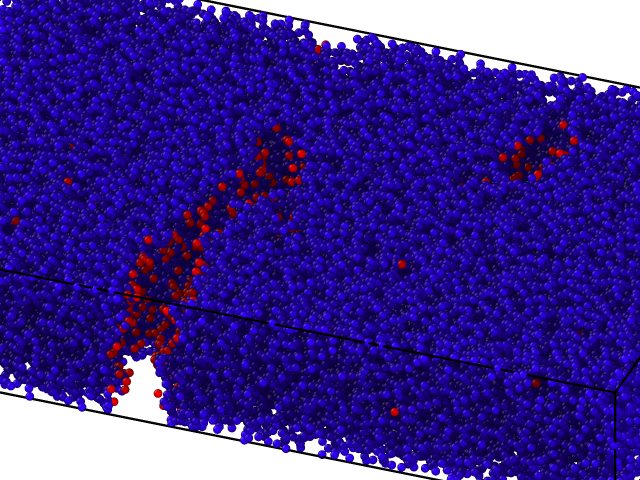
\includegraphics[width=8cm, height=6cm]{crack_vol.png}
    \caption{Atoms in red are those with Voronoi cell volume $v_i>0.042$~nm$^3$.  The voids represent fractures.}
    \label{fig:crack_vol}
    \end{figure}



The most straightforward way of defining ground truth is a dummy indicator variable $\phi_i(t) \in\{0,1\}$, specifying whether or not an atom $i$ is part of a fracture at time $t$. Given a system with $n$ atoms, $\boldsymbol{\phi}(t)$ is a binary vector of length $n$. An important consideration, however, is that the simulation data described in previous sections does not directly give ground truth information. Instead, the ground truth must be extracted from the simulation output.


    
In order to establish the ground truth, we set the threshold value for a given time $t$ to be equal to three standard deviations above the mean Voronoi cell volume at that time.  Thus, we define a normalized cell volume and test whether it is greater than 3:
    \begin{equation}
    \hat{v}_i(t) = \frac{v_i(t) - \mu_v(t)}{\sigma_v(t)} > 3,
    \end{equation}
where $\mu_v(t)$ is the mean and $\sigma_v(t)$ is the standard deviation of $v_i(t)$ over all $i\in\{1,\dots,n\}$.  Note that in the postprocessed nucleation data supplied with the LAMMPS simulation data, this is equivalent to testing whether the quantity in the field {\tt nuc\_v} exceeds 1.

Because of the effects of free surfaces discussed in Section~\ref{subsec: Physical Features} above, $v_i(t)$ must be modified to disregard cell volumes that are large because they are on the boundary of a surface rather than a fracture.  Since these cell volumes do not significantly change over time, we define a new quantity that subtracts out the $t=0$ value, $v'_i(t) = v_i(t)-v_i(0)$, and instead test whether
\begin{equation}
    \label{eqn: cell volume}
    \hat{v}'_i(t) = \frac{v'_i(t) - \mu_{v'}(t)}{\sigma_{v'}(t)} > 3.
\end{equation}
The ground truth can then be defined:
\begin{equation}
    \label{eqn: ground truth}
    \phi_i(t) = \begin{cases}
      0 & \text{if }\hat{v}'_i(t) \le 3 \\
      1 & \text{if }\hat{v}'_i(t) > 3 \\
    \end{cases} 
\end{equation}

We apply two further corrections to $\phi_i(t)$, to limit the case of false negatives (where atoms on the boundary are identified as $\phi_i(t)=0$) as well as false positives (where atoms not on the boundary of a fracture are identified as $\phi_i(t)=1$).

The false negative case occurs when an atom is at the boundary of a fracture, but is surrounded by a sufficient number of other nearby atoms that its Voronoi cell volume does not extend out into the void.  To account for this, we consider a small neighborhood around each positively identified atom $i$.  Any other atom whose path length to $i$ consists of fewer than a small number of edges (such as 2 or 3) is considered to be on the boundary as well.

The false positive case occurs early in the simulation, prior to nucleation, when the standard deviation $\sigma_{v'}(t)$ is very small, and atoms can be identified as positive purely due to spatial fluctuations in density.  To reduce this problem, we use the fact that an atom on the boundary of a fracture at time $t$ is expected to remain on the boundary of a fracture for the remainder of the simulation.  If an atom is positively identified, we test whether it remains positively identified for the majority of the remaining simulation times.  If not, it is not considered to be on the boundary.

\subsection{Cell Volume as Indicator of Fracture Face}

We propose an alternative way to extracting information from simulations on whether an atom is at a fracture boundary, and then training our algorithms using this ground truth.  Instead, we can simply adopt the cell volumes as ground truth, and train our algorithms to predict this.  Our predictions may then be post processed using Equations~(\ref{eqn: cell volume}) and (\ref{eqn: ground truth}) to determine which atoms are at fracture boundaries.  This could have the advantage of providing a more objective prediction, but involves solving a regression problem rather than merely a classification problem.

\subsection{Indicator of Large Sized Ring}

        %%  LOOP20 AND FRACTURE NUCLEATION FIGURE 
    \begin{figure}
    \begin{subfigure}{.5\textwidth}
      \centering
      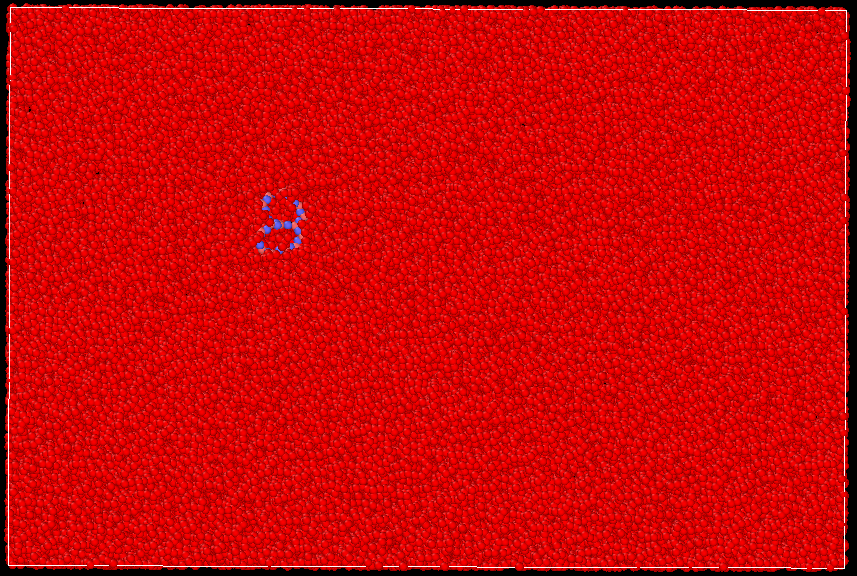
\includegraphics[width=.8\linewidth]{images/fp1_ini_ring20_t=604.png}
      \caption{Initial appearance of a large ring at t = 1,208,000}
      \label{fig:loopfig1}
    \end{subfigure}%
    \begin{subfigure}{.5\textwidth}
      \centering
      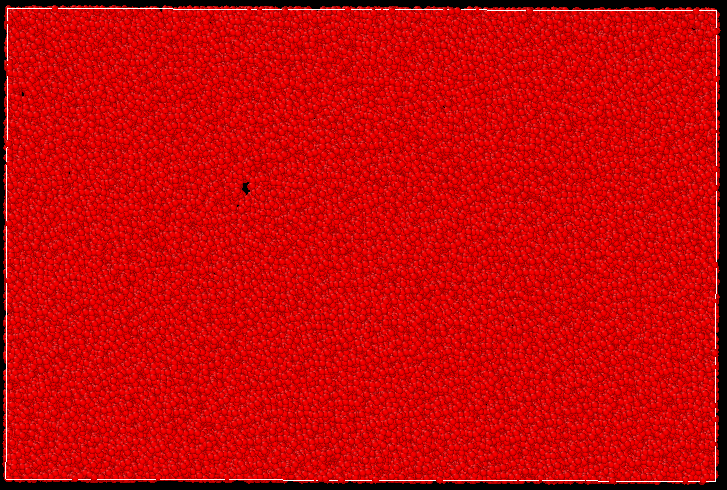
\includegraphics[width=.8\linewidth]{images/fp1_ini_nucle_t=619.png}
      \caption{Initial fracture nucleation appears at t = 1,238,000}
      \label{fig:loopfig2}
    \end{subfigure}
    \begin{subfigure}{.5\textwidth}
      \centering
      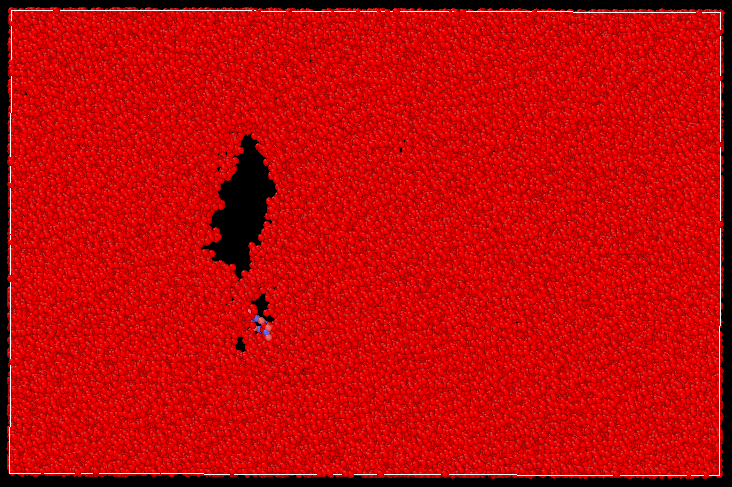
\includegraphics[width=.8\linewidth]{images/fp1_propa.png}
      \caption{Large rings appear along with fracture propagation}
      \label{fig:loopfig3}
    \end{subfigure}
    \begin{subfigure}{.5\textwidth}
      \centering
      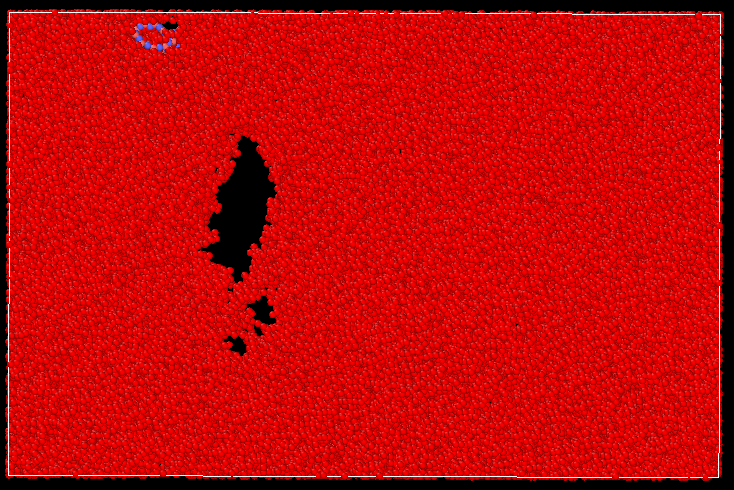
\includegraphics[width=.8\linewidth]{images/fp1_propa2.png}
      \caption{Large rings appear along with new nucleation}
      \label{fig:loopfig4}
    \end{subfigure}
    
    \caption{Four snapshots showing the relationship between large ring structure and fracture nucleation/propagation behavior.  {\color{red}NOTE: Earlier, we define $t$ to be the snapshot number, not the simulation time step, so be sure to change the figure captions to this notation.  Also, don't omit the time step information for (c) and (d).}}
    \label{fig:loopfig}
    \end{figure}
    
    As we previously discussed in section \ref{subsec: Features} that the sizes of rings, defined as lengths of cycle consisting of alternating Si and O atoms, has been observed to correlate with fracture behavior, we use an alternative potential indicator of fracture nucleation using rings of size 20. So, we can also define the ground truth as a dummy indicator variable $\phi_i(t) \in\{0,1\}$, specifying whether or not an atom $i$ has ever been part of a ring of size 20 during all simulation steps. {\color{red}Explain why size 20 and not some other size.}
    
    Figure \ref{fig:loopfig} helps explain intuition behind this observation. As figure \ref{fig:loopfig1} shows, a large ring appears in the material. And inside the ring, there is a large void. As tensile is applied, the large void is more likely to deform and eventually lead to fracture. As the figure \ref{fig:loopfig2} shows, a fracture nucleates where the large ring appears. Not only does large rings relate to fracture nucleation, they are also related to fracture propagation. Figure \ref{fig:loopfig3} indicates appearance of large rings along with direction that the existing fracture propagates. Figure \ref{fig:loopfig4} shows that a large ring also appears when new fracture nucleates when there is existing fracture.

    The advantage of this definition is that in such a way, this indicator is less arbitrary. However, the disadvantage is that the number of large rings is very small compared to other smaller-sized rings. For example, in one simulation, only 423 out of around 70000 atoms are part of a 20-sized ring. This worsens the imbalanced classes issue and thus creates a modelling challenge to tackle this problem. {\color{red}But you haven't yet explained why there is a class imbalance in the first place.  Maybe this is the right place to do so?}



\section{Machine Learning Methods}

{\color{red}Is this section still accurate?  The preliminary results that follow use methods that are different from the ones here.  Do you still plan on using bagging and boosting, for instance?  The RNN method is clearly relevant, and I hope we will use some form of it soon, so that part is worth keeping.}

The objective of this project is to produce a surrogate model of the molecular dynamic simulations using supervised machine learning techniques. We are addressing our two goals listed in Section~\ref{sec: Goals} with two methods, respectively. First, we use ensemble methods such as random forest to predict nucleation at a fixed future time step, given feature information at $t=0$.

Second, we use a recurrent neural network (RNN) with the long-short term memory (LSTM) mechanism, to learn the dynamic process of fracture propagation.

\subsection{Random Forest for Predicting Fracture Nucleation}

%Random forest. Boosting, bagging. 
For the purpose of determining whether or not a node is associated with a fracture, we are implementing ensemble-based ML methods. The goal of ensemble methods is to take predictions made by a subset of features, and combine them into one single learned estimator. With our feature set being quite large, ensemble methods may be a useful means to predict fracture labels. 

Core ensemble methods include bagging (bootstrap aggregating) and boosting. A ``bagged'' random forest method is generated by creating a tree from features randomly drawn with replacement. 
% Since our representation is graph-like these trees make sense logically. 

Our bagging algorithm works as follows:

\begin{enumerate}
\item Take training set $T$ with $N$ features.
\item Create $n$ models $\{L_1,\dots,L_n\}$.
\item For model $L_i$, create a training set by choosing $d_i<N$ features from $T$ with replacement, and train the model.
\item Determine the output of the algorithm by majority vote among the $n$ models.
\end{enumerate}

Adaboost (adaptive boosting), on the other hand, is a boosting method that learns from previous mistakes made during training. By doing so, the model can increase the weights of incorrectly predicted points from the training data.

Our boosting algorithm works as follows:

\begin{enumerate}
    \item Initialize weights for each individual feature.
    \item Train a classifier on each individual feature.
    \item Find the weighted misclassification (error) rate.
    \item Update feature weights based on this error.
    \item Repeat until error is minimized.
\end{enumerate}


\subsection{Fracture Propagation}
%RNN, 

\begin{figure}[!b]
    \centering
    \noindent
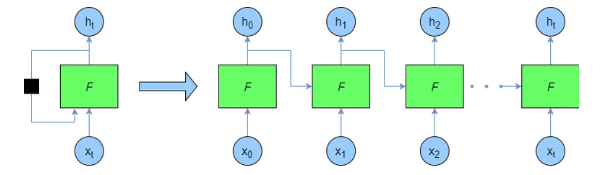
\includegraphics[width=12cm , height = 5cm]{images/rnn.PNG}
    \caption{Representation of a Recurrent Neural Network}
    \label{fig:rnn}
\end{figure}

Due to the dynamical nature of our graph changing over each time step, we will be implementing an RNN to predict the ground truth at each time step. An illustration of the basic RNN architecture is shown in Figure~\ref{fig:rnn}.  The main idea behind an RNN is that it trains on an entire time series, learning the dynamics of a process which it stores using a ``memory'' of internal states.  The LSTM mechanism is a refinement of this memory, allowing the neural network to give added weight to information learned in more recent time steps.

The training input to our RNN will be a time series of graphs based on simulation data, where nodes will be labeled with the full set of feature values described in Section~\ref{subsec: Features}.  For every time $t$, the RNN uses the (appropriately weighted) information from that and all previous times to output feature and ground truth values for time $t+1$.  These are compared with simulation results, from which a loss function is calculated and the internal neural network weights are updated.

Once the RNN is trained and its weights are set, it is used for prediction.  Unlike in the training phase, the input in the prediction phase is simply the $t=0$ feature values.  The output is a time series of graphs, giving the full predicted evolution of features and ground truth.

Recall that certain of our features, such as atom displacement and active atoms, are undefined at $t=0$ and thus meaningful only as part of the training process.  Others, however, are well-defined at any individual time step.
\newpage
The proposed architecture is as follows:
\bigskip
\begin{center}
\tikzstyle{decision} = [diamond, draw, fill=blue!20, 
    text width=4.5em, text badly centered, node distance=3cm, inner sep=0pt]
\tikzstyle{block} = [rectangle, draw, fill=blue!20, 
    text width=5em, text centered, rounded corners, minimum height=4em]
\tikzstyle{line} = [draw, -latex']
\tikzstyle{cloud} = [draw, ellipse,fill=red!20, node distance=3cm,
    minimum height=2em]
    
\begin{tikzpicture}[node distance = 2cm, auto]
    % Place nodes
    \node [block] (init) {MD Simulation Data};
    \node [block, below of=init] (features) {Extracted Features};
    \node [block, below of=features] (training) {Training Set};
    \node [block, left of=training, node distance=3cm] (test) {Test Set};
    \node [block, right of=training, node distance=3cm] (validate) {Validation Set};
    \node [decision, below of = training] (RF) {Random Forest};
    \node [decision, below  of = test] (rnn) {LSTM};
    \node [cloud, below of = RF] (out) {Surrogate Model};
    %\node [cloud, below of= RF, node distance=3cm] (pof) {RF Output};
    %\node [cloud, below of= rnn, node distance=3cm] (rnnout) {RNN Output};

    % Draw edges
    \path [line] (init) -- (features);
    \path [line] (features) -- (validate);
    \path [line] (features) -- (training);
    \path [line] (features) -- (test);
    \path [line] (training) -- (RF);
    \path [line] (training) -- (rnn);
    \path [line] (rnn) -- (out);
    \path [line] (RF) -- (out);
    \path [line] (validate) |- node [near end] {} (out);
\end{tikzpicture}
\end{center}

\begin{enumerate}
    \item Analyze and determine features from the MD data.
    \item Extract the features and prepare data for training.
    \item Split the dataset into three sets: training, validation, and test
    \item
    \begin{enumerate}
        \item Train the training set using Random Forest to predict which atoms are part of a fracture.
        \item Train the data using LSTM to predict fracture evolution.
    \end{enumerate}
    \item Validate surrogate model using validation set.
    \item Feature analysis. Fine tune features which are deemed most important. 
    \item Finalize surrogate model on test set. 
\end{enumerate}